\documentclass[../main.tex]{subfile}
\graphicspath{{\subfix{../images}}}
\begin{document}

我们正在见证视觉界的快速、革命性的变化,主要是由深度卷积神经网络(CNN)[1]和大规模训练数据的可用性[2]引起的。基于深度网络的方法最近在图像分类[3]、[4]、[5]、[6]、物体检测[7]、[8]、[5]、许多其他识别任务[9]、[10]、[11]、[12],甚至非识别任务方面的技术水平上有了很大提高。

\begin{figure}[htb]
    \centering
    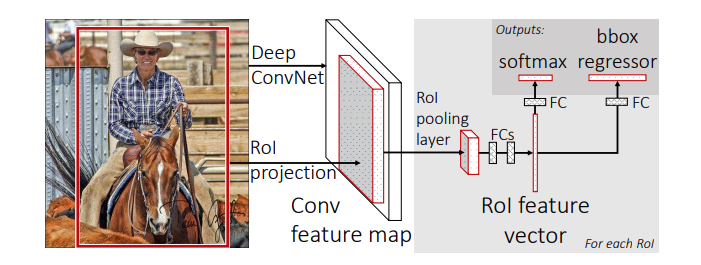
\includegraphics[width=\textwidth]{fig1.png}
    \caption{顶部:裁剪或扭曲以适应固定尺寸。中间:一个传统的CNN。底部:我们的空间金字塔集合网络结构。}
    \label{fig:fig1}
\end{figure}

然而,在CNN的训练和测试中存在一个技术问题:普遍的CNN需要一个固定的输入图像尺寸(如224×224),这就限制了输入图像的长宽比和比例。当应用于任意尺寸的图像时,目前的方法大多通过裁剪[3]、[4]或扭曲[13]、[7]将输入图像适配到固定尺寸,如图\ref{fig:fig1}(顶部)所示。但是裁剪的区域可能不包含整个物体,而扭曲的内容可能导致额外的的几何变形。由于内容的损失或失真,识别的准确性可能会受到影响。此外,当物体的尺度变化时,预先定义的尺度可能不适合。固定输入尺寸忽略了涉及尺度的问题。

那么,为什么CNN需要一个固定的输入大小呢?一个CNN主要由两部分组成:卷积层和后面的全连接层。卷积层以滑动窗口的方式运作,并输出代表激活的空间排列的特征图(图\ref{fig:fig2})。事实上,卷积层不需要固定的图像尺寸,可以生成任何尺寸的特征图。另一方面,全连接层根据其定义需要有固定大小/长度的输入。因此,固定尺寸的约束只来自全连接层,它存在于网络的更深阶段。

\begin{figure}[htb]
    \centering
    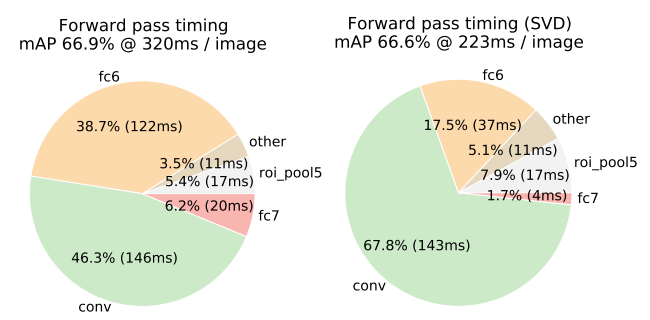
\includegraphics[width=\textwidth]{fig2.png}
    \caption{特征图的可视化。(a) Pascal VOC 2007中的两幅图像。(b) 一些$\text{conv}_5$过滤器的特征图。箭头表示最强的反应和它们在图像中的相应位置。(c) 相应过滤器反应最强的ImageNet图像。绿色的矩形标志着最强反应的感受区。}
    \label{fig:fig2}
\end{figure}

在本文中,我们介绍了空间金字塔池化(SPP)[14], [15]层来消除网络的固定尺寸约束。具体来说,我们在最后一个卷积层的顶部添加一个SPP层。SPP层汇集特征并产生固定长度的输出,然后将其送入全连接的层(或其他分类器)。换句话说,我们在网络层次结构的较深阶段(卷积层和全连接层之间)进行一些信息 "聚合",以避免一开始就进行裁剪或扭曲。图\ref{fig:fig1}(底部)显示了引入SPP层后网络结构的变化。我们称这种新的网络结构为SPP-net。

空间金字塔集合[14], [15](俗称空间金字塔匹配或SPM[15]),作为语料袋(BoW)模型[16]的延伸,是计算机视觉中最成功的方法之一。它将图像划分为从精细到粗糙的层次,并将局部特征聚集在其中。在最近CNN盛行之前,SPP长期以来一直是分类(如[17]、[18]、[19])和检测(如[20])的领先和竞赛获奖系统的关键组成部分。然而,SPP还没有在CNN的背景下被考虑。我们注意到,SPP对于深度CNN来说有几个显著的特性。1)SPP能够无视输入尺寸而产生一个固定长度的输出,而之前的深度网络[3]中使用的滑动窗口池化不能;2)SPP使用多级空间分块,而滑动窗口池只使用单一的窗口大小。多级池化已被证明对物体变形具有鲁棒性[15];3)由于输入尺度的灵活性,SPP可以汇集在不同尺度上提取的特征。通过实验我们表明,所有这些因素都提升了深度网络的识别精度。

SPP-net不仅可以从任意大小的图像/窗口中生成表征用于测试,而且还允许我们在训练过程中输入不同大小或比例的图像。用不同尺寸的图像进行训练可以增加尺度不变性并减少过拟合。我们开发了一种简单的多尺寸训练方法。对于一个接受可变输入尺寸的单一网络,我们用共享所有参数的多个网络来近似它,而这些网络中的每一个都用固定的输入尺寸进行训练。在每个历时中,我们用一个给定的输入尺寸训练网络,并在下一个历时中切换到另一个输入尺寸。实验表明,这种多尺寸训练和传统的单尺寸训练一样收敛,并能带来更好的测试精度。

SPP的优势与具体的CNN设计是正交的。在ImageNet 2012数据集的一系列控制变量实验中,我们阐明了对于现有的四个典型模型[3],[4],[5](或它们的变种),SPP相较于对应的无SPP版本,对所有模型都有所提升。这些架构有不同的卷积核数量/大小、步长、深度或其他设计。因此,我们有理由猜测,SPP应该能改善更复杂(更深更大)的卷积结构。SPP-net在Caltech101[21]和Pascal VOC 2007[22]上也显示了最先进的分类结果,并只使用了单一完整的图像表示,没有进行微调。

SPP-net在物体检测方面也显示出巨大的优势。在领先的物体检测方法R-CNN\cite{rcnn}中,候选窗口的特征是通过深度卷积网络提取的。这种方法在VOC和ImageNet数据集上都表现出了显著的检测精度。但是R-CNN中的特征计算是很耗时的,因为它对每张图像的数千个扭曲区域的原始像素反复应用深度卷积网络。在本文中,我们表明我们可以在整个图像上只运行一次卷积层(不管窗口的数量如何),然后通过SPP-net在特征图上提取特征。这种方法产生的速度比R-CNN快一百多倍。请注意,在特征图(而不是图像区域)上训练/运行检测器实际上是一个更流行的想法[23], [24], [20], [5]。但是SPP-net继承了深度CNN特征图的力量,同时也继承了SPP在任意窗口大小上的灵活性,这就导致了出色的准确性和效率。在我们的实验中,基于SPP-net的系统(建立在R-CNN管道上)计算特征的速度比R-CNN快24-102倍,同时具有更好或相当的准确性。利用EdgeBoxes[25]最近的快速提议方法,我们的系统处理一幅图像(包括所有步骤)只需0.5秒。这使得我们的方法对现实世界的应用很实用。

本稿件的初步版本已经发表在ECCV 2014上。基于这项工作,我们参加了ILSVRC 2014的比赛[26],在所有38个团队中,物体检测排名第2,图像分类排名第3(均为只提供数据的赛道)。我们为ILSVRC 2014做了一些修改。我们表明,SPP网络可以提升各种网络的深度和规模(第3.1.2-3.1.4节),超过无SPP的对应网络。此外,在我们的检测框架的驱动下,我们发现对具有灵活位置/大小的窗口的特征图进行多视图测试(第3.1.5节)可以提高分类精度。本稿件也提供了这些修改的细节。

\end{document}